
\documentclass[11pt]{article}
% \usepackage[margin=1in]{geometry}
\usepackage{enumerate}
\usepackage{forest}
\usepackage[margin=1in]{geometry}
\usepackage{mathtools}
\usepackage{amsmath}
\usepackage{amssymb}
\usepackage{gensymb}
\usepackage{hyperref}
\usepackage{floatrow}
\floatsetup[table]{capposition=top}

%opening
\title{CSCI 491/591 P2}
\date{March 1, 2016}
\author{Group 4\\Chenglin Fan, Jici Huang,
Angelica Davis, Peng Zou}

\begin{document}

\maketitle
\noindent
In this project our team is exploring a series of data sets comprised of GPS trajectories collected from taxi 'trips' around various major cities across the globe. In the award winning paper, "Efficient Map Reconstruction and Augmentation via Topological Methods" by Wang et. all, these GPS trajectories were processed using two critical topological techniques in order to construct an accurate image of the road networks of these major cities. Much of the strength of this paper comes from the reconstruction process's robustness against noise. The end goal of our project is to deeply understand the topological concepts and techniques used in the paper, and to add to our skill sets a particularly powerful data processing technique against multiple kinds of noise that are common in real data sets. 

For this deliverable, we have selected an interesting data set, the GPS trajectories of Berlin, among several others that we would like to explore in the project. In this document we will provide the information on where the data set is from and explain the meaning of the collected data. We will also conjecture what we might find in the exploration of the data set in addition to digging into the map reconstruction processes.
\section*{Data Set Selection}
As mentioned above, the data set that will be explored in depth for this project is the collection of GPS trajectories taken from the German city, Berlin.
%In P1, we went through all data sets provided by Map Construction Portal and we decided to investigate trajectory data of the tracks in Berlin, large. 
The team decided it was a suitable representative data set since the size of the data is about midway between that of Chicago and Athens (two of the other trajectory data sets). The size of data set is a reasonable characteristic for comparison because each of the data sets represent overlapping trajectories as well as noisy trajectories. Thus, a mid-sized data set may well represent the noise ratio (either due to noisy trajectories or the lack of sampling uniformity). %In addition (I suspect but will fact check my memory tommorrow) based on the visual appearances of each of the respective road maps, each city has a comparable amount of sprawl and order in their layouts. From this we conjecture that the noise introduced from the GPS instrumentation itself will not play a major role in the overall performance of the techniques applied.
% Data set choice (8 points). You must select an interesting data set
% that you will investigate in this project. The data set can be real (GPS trajectories,
% Four-square check-ins, gene expressions, March madness brackets,
% baseball statistics, 3D objects, movie scripts, etc.), or it can be theoretical
% (flip graphs, the space of image patches, etc.). [Deliverable: one-to-two page write-up].

\section*{Details About the Data}
The Berlin GPS trajectories dataset was downloaded from the Map Construction Portal (\url{http://www.mapconstruction.org/data_downloads/}). 
The GPS trajectories of Berlin data set contains the trajectory data of taxi trips in Berlin. Here the trip is a collection of GPS trajectories that describe one path traveled over some time period. The trajectory data has more than 27,000 trips in .txt format. \\
Each trip file consists of a series trajectories each represented by an x-coordinate, y-coordinate and a time stamp corresponding to the x, y-coordinate location at that particular time. Table \ref{table:questions} provides a small sample of a trip file taken from the trajectory data of Berlin.
% Explain where the data is
% from, what the data means,
% TODO: write something here.\\
% \begin{center}
%  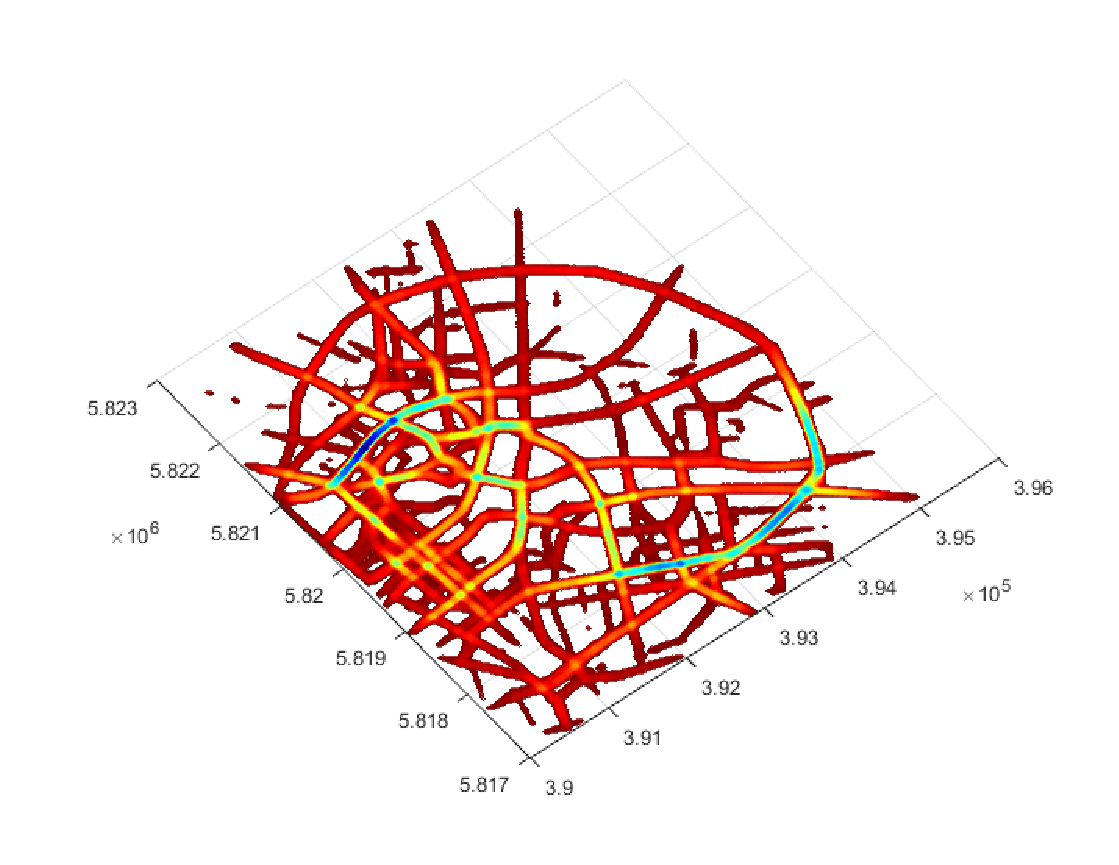
\includegraphics[scale=0.9]{p1.eps} 
% \end{center}
\begin{table}
\begin{center}
\begin{tabular}{ |c |c| r| }
\hline
  x & y & Time stamp   \\ \hline
  393742.586772 & 5821049.184616 & 2585542.00   \\ \hline
  393747.949682 & 5821296.284551 & 2585604.00 \\  \hline
  393883.091662 & 5821448.203015 & 2585677.00  \\ \hline
  393759.343945 & 5821821.259046 & 2585738.00\\ \hline
  \vdots & \vdots & \vdots \\ \hline
\end{tabular}
\end{center}
\caption{An excerpt of trajectory data of Berlin in a trip file}
\label{table:questions}
\end{table}

%\begin{figure}[h!]
 % \caption{A tracking map after processing the track Berlin large data set}
 % \centering
% 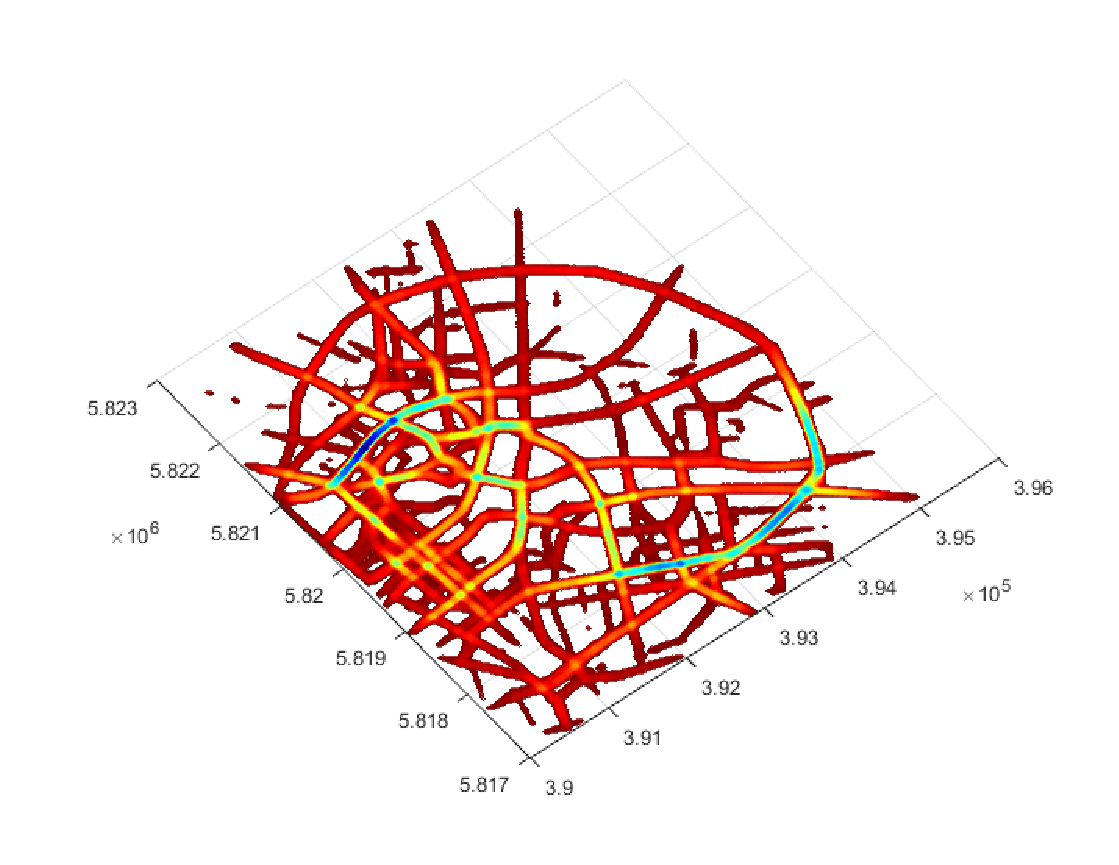
\includegraphics[scale=0.8]{p1.eps} 
%\end{figure}

\pagebreak
\section*{Exploration} 
%We might find out that the trajectory data we chose does not produce any map without using the techniques we mentioned in the previous deliverable. We might come up with a road map of Berlin based on the trajectory data we chose after using the techniques. We might find some new technique by exploring the GPS trajectories data.
The items we will explore in this data set are as follows: 
\begin{itemize}
	\item Estimate the underlying road network  by using the trajectory data.\\ 
	As described above, the trajectory data is a compilation of taxi trips around a major city. As a real world event the complete path of a taxi trip is unpredictable, and the complete data set is comprised of overlapping trajectories. With this in mind, the raw data could be imagined as a monochromatic drip painting of the city. Since the web of trajectories stretches out in any direction with virtually indistinguishable overlaps, it will not be immediately clear from the trajectory data where the distinct roads occur. Therefore it will be necessary to apply some simplification to introduce more clarity into the image. This will be done by analyzing the most topologically persistent features, and removing the data not associated with these features.%, as the trajectory data record the track of taxis, which usually run on the road network of the city.
	
	\item  Find the roads with heavy traffic, namely the roads with high density of trajectory.   We also want to analyze the topological structure of the heavy roads in the city.
\end{itemize}
% \section*{Discussion}
% In P2, we had discussion on the analysis of the data. We came up with two data files from the original trip files. \\
% It is usually nice to conclude any write-up.\\

% pts.txt: grid points after the city, 
% manifold value: clr.txt
\section*{Conclusion}
%Our group believes that the project is interesting. We are motivated to explore the GPS data by the applications of GPS that are affecting every aspect of modern life. We want to use the topology knowledge in this class to do some thing with application in real life.
In this project, our group will explore the GPS trajectory data of Berlin in Germany. We aim to construct an image of the road network using this data. Since the collected data is real, its raw form has little organization that would be immediately helpful in identifying distinct roads. Therefore we will be applying the topological techniques used in the map reconstruction paper. From this process, our group hopes to gain a deeper understanding of these topological concepts and at the same time learn how to process real, noisy data sets.

% \\
% 1. Using a. b. c. ... as section numbers is not really standard, and looks a little funny to me.  Perhaps just stick with the standard Section Name (maybe you were using an enumeration instead)?{\bfseries FIXED}\\ 
% Use capital letters to start a sentence (e.g., "the description of map data ..."){\bfseries FIXED}\\
% This deliverable was expected to be a bit more narrative in nature.  As it is written, it is closer to an outline than a write-up.\\
% For vertex data: what are the coordinates?  lat/lon or x/y (if lat/lon, you will need to use a local projection to the plane ...)\\
% 'track data' $\rightarrow$ 'trajectory data'\\
%  Captions for tables should always go above the table (for figures, it always goes below the figure).  See this reference: The Elements of Typographic Style){\bfseries FIXED}\\
% While HZ02 is one of the first references on persistence, also take a look at the survey paper: https://users.cs.duke.edu/~edels/Papers/2008-B-02-PersistentHomology.pdf\\
% c.1 and d.1: Persistent is an adjective, so either write "persistent homology" or "persistence" \\
% discrete Morse theory differs from Morse theory in that we no longer require differentiable functions.\\
% Perhaps a description of what is done in [SL15] would be in order.
% Your biblio entries are a little off.  Please check your .bib file (if you don't see why ... send me your .bib file and I can take a look for you).\\
% Are you assuming a manifold somewhere?  I ask because you talk about manifolds ...{\bfseries NA}\\
% Be sure to have your group number in your project deliverables.{\bfseries FIXED}\\
\end{document}
